\subsubsection{UC12 - Validazione nuovo account registrato}
\begin{figure}[h]
	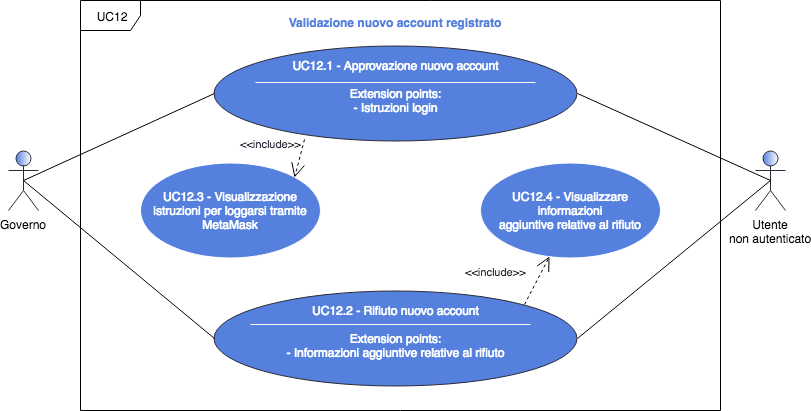
\includegraphics[width=15.5cm]{res/images/UC12Validazione.png} %da adattare in larghezza
	\centering
	\caption{UC12 - Validazione nuovo account registrato}
	
\end{figure}
\begin{itemize}
	\item \textbf{Attori Primari}:
	governo;
	\item \textbf{Attori Secondari}:
	utente non autenticato;
	\item \textbf{Descrizione}: l'account utente può venire rigettato o approvato dal governo;
	\item \textbf{Scenario principale}: l'utente si è registrato al sistema ma è ancora in attesa di una risposta da parte del governo in merito alla validazione del proprio account. Il flusso degli eventi è il seguente:
	\begin{itemize}
		\item il governo ottiene la lista delle aziende in lista di attesa [UC11.3] o dei cittadini in lista di attesa [UC11.4];
		\item il governo approva [UC12.1] o rifiuta [UC12.2] la richiesta di iscrizione;
	\end{itemize}
	\item \textbf{Precondizione}: l'utente è in coda di attesa per la validazione dell'account;
	\item \textbf{Postcondizione}: l'account utente viene approvato o rigettato. 
\end{itemize}
\subsubsection{UC12.1 - Approvazione nuovo account}
\begin{itemize}
	\item \textbf{Attori Primari}:
	governo;
	\item \textbf{Attori Secondari}:
	utente non autenticato;
	\item \textbf{Descrizione}: l'account utente viene approvato;
	\item \textbf{Scenario}: in seguito alla registrazione, il governo riconosce validi i dati immessi dall'utente;
	\item \textbf{Inclusioni}:
	\begin{itemize}
		\item \textbf{UC12.3}: in seguito all'approvazione dell'account, l'utente visualizza una breve e concisa guida su come loggarsi al sito;
	\end{itemize}
	\item \textbf{Precondizione}: l'utente ha portato a termine la richiesta di registrazione ed è ancora in attesa di verifica;
	\item \textbf{Postcondizione}: l'utente è stato verificato e può visualizzare il modo corretto per eseguire il login alla piattaforma.
	
\end{itemize}
\subsubsection{UC12.2 - Rifiuto nuovo account}
\begin{itemize}
	\item \textbf{Attori Primari}:
	governo;
	\item \textbf{Attori Secondari}:
	utente non autenticato;
	\item \textbf{Descrizione}: l'account utente viene rifiutato;
	\item \textbf{Scenario}: in seguito alla registrazione, il governo riconosce non validi i dati immessi dall'utente;
	\item \textbf{Inclusioni}:
	\begin{itemize}
		\item \textbf{UC12.4}: in seguito al rigetto  dell'account, l'utente visualizza dettagli aggiuntivi del perchè non è stato accettato;
	\end{itemize}
	\item \textbf{Precondizione}: l'utente ha portato a termine la richiesta di registrazione ed è ancora in attesa di verifica;
	\item \textbf{Postcondizione}: l'utente risulta rifiutato e riceve le informazioni relative a tale rifiuto.
	
\end{itemize}
\subsubsection{UC12.3 - Visualizzazione istruzioni per loggarsi tramite MetaMask\glosp}
\begin{itemize}
	\item \textbf{Attori Primari}:
	governo;
	\item \textbf{Attori Secondari}:
	utente non autenticato;
	\item \textbf{Descrizione}: l'utente, durante il primo tentativo di accesso alla piattaforma dopo l'approvazione dell'account, visualizza una guida contenente le istruzioni per procedere al login tramite MetaMask\glosp;
	\item \textbf{Scenario}: in seguito all'approvazione dell'account, l'utente cerca di effettuare il suo primo login, e gli vengono fornite tutte le istruzioni necessarie;
	\item \textbf{Precondizione}: l'utente è stato verificato e tenta di eseguire per la prima volta il login;
	\item \textbf{Postcondizione}: l'utente possiede le conoscenze necessarie al fine di conseguire un login corretto e sicuro tramite il plugin MetaMask\glosp.
\end{itemize}
\subsubsection{UC12.4 - Visualizzazione informazioni aggiuntive in merito al rigetto dell'account}
\begin{itemize}
	\item \textbf{Attori Primari}:
	governo;
	\item \textbf{Attori Secondari}:
	utente non autenticato;
	\item \textbf{Descrizione}: l'utente visualizza le informazioni aggiuntive relative al rigetto del proprio account;
	\item \textbf{Scenario}: in seguito al rifiuto dell'account, l'utente riceve le informazioni relative a tale rigetto da parte del governo;
	\item \textbf{Precondizione}: l'utente non ha idea del perchè non è stato accettato;
	\item \textbf{Postcondizione}: l'utente riconosce di aver inserito dati falsi o contenenti errori, pertanto dovrà riprovare la registrazione.
\end{itemize} 
\subsubsection{UC13 - Rimborso IVA}
\begin{itemize}
	\item \textbf{Attori Primari}:
	governo;
	\item \textbf{Attori Secondari}:
	azienda, MetaMask\glo;
	\item \textbf{Descrizione}: il governo rimborsa l'IVA ad un'azienda che risulta in stato di credito al momento del saldo trimestrale;
	\item \textbf{Scenario}: dopo aver visualizzato lo stato dell'IVA di un'azienda [UC11.2.1] il governo decide di effettuare il rimborso cliccando sul pulsante dedicato. Dovrà confermare la transazione attraverso il plugin MetaMask\glo;
	\item \textbf{Estensioni}: 
	\begin{itemize}
		\item \textbf{UC7.5}: l'utente tenta il pagamento ma l'esito non va a buon fine. La causa del fallimento dell'operazione è gestito dal plugin stesso.
	\end{itemize}
	\item \textbf{Inclusioni}: 
	\begin{itemize}
		\item \textbf{UC11.2}: l'utente per poter accedere al pulsante per il rimborso dell'azienda deve visualizzare la lista delle aziende verificate;
	\end{itemize}
	\item \textbf{Precondizione}: il sistema ha mostrato la lista delle aziende già verificate, con il relativo stato dell'IVA. L'utente ha premuto il pulsante per il rimborso e confermato l'operazione;
	\item \textbf{Postcondizione}: il sistema avvisa l'utente che l'operazione è avvenuta con successo. Il rimborso è stato versato all'azienda.
\end{itemize} 
